\section{Literature Review}

\subsection{Related Works: Existing Products and Technologies}

\begin{enumerate}


\item{\bf{PARO}}
\vspace{0.25cm}

PARO, a robotic baby seal developed by the National Institute of Advanced Industrial Science and Technology (AIST) in Japan, is one of the most well-known emotional support robots. It is designed to provide companionship to elderly individuals, particularly those with dementia or cognitive impairments. PARO incorporates several advanced features to enhance its therapeutic effectiveness: it is equipped with tactile sensors that allow it to respond to touch, microphones to recognize voices and sounds, and artificial intelligence to learn and adapt to the user’s preferences over time. It also has movement and behavior patterns that mimic a real seal, such as blinking its eyes, moving its flippers, and making sounds, which helps in creating a comforting and engaging interaction. Studies have shown that PARO can reduce stress and anxiety, increase socialization, and improve overall mood among users \cite{wada2006}.

\begin{figure}[ht]
    \centering
    
\includegraphics[width=\textwidth]{paro.png}
    \caption{PARO, baby seal robot adapted from \cite{shibata2021}}
    \label{fig:paro}
\end{figure}

\item{\bf{Therabot}}
\vspace{0.25cm}

Therabot is a robot designed to engage users in therapeutic interactions by responding to their emotions through computer vision and providing appropriate feedback, helping individuals process their feelings and improve their mood. It features a soft-textured exterior, which participants have expressed a strong preference for, as it creates a sense of safety and emotional support, making the robot more approachable and pleasant to interact with. Additionally, the integration of a mobile app allows for more interactive and personalized sessions, enhancing user engagement and providing a more beneficial therapeutic experience \cite{bethel2018}.

\begin{figure}[ht]
    \centering
    
\includegraphics[width=\textwidth]{therabot.jpg}
    \caption{Therabot, the robotic beagle puppy adapted from \cite{therabot2024}}
    \label{fig:therabot}
\end{figure}

\newpage
\item{\bf{Pepper}}
\vspace{0.25cm}

Pepper is a humanoid robot designed to recognize emotions through facial expressions, vocal tones, and body language, enabling empathetic interactions in both personal and business settings. Using natural language processing (NLP), it engages in conversations and tailors its responses based on context and past interactions. Pepper features 360-degree mobility, an interactive touchscreen, and cloud-based AI for real-time updates. It integrates with business systems, making it versatile for retail, healthcare, and education, where it assists with tasks like greeting customers, monitoring patients, and engaging children. Customizable and adaptive, Pepper excels as an emotional support and service robot \cite{softbank2022}.

\begin{figure}[ht]
    \centering
    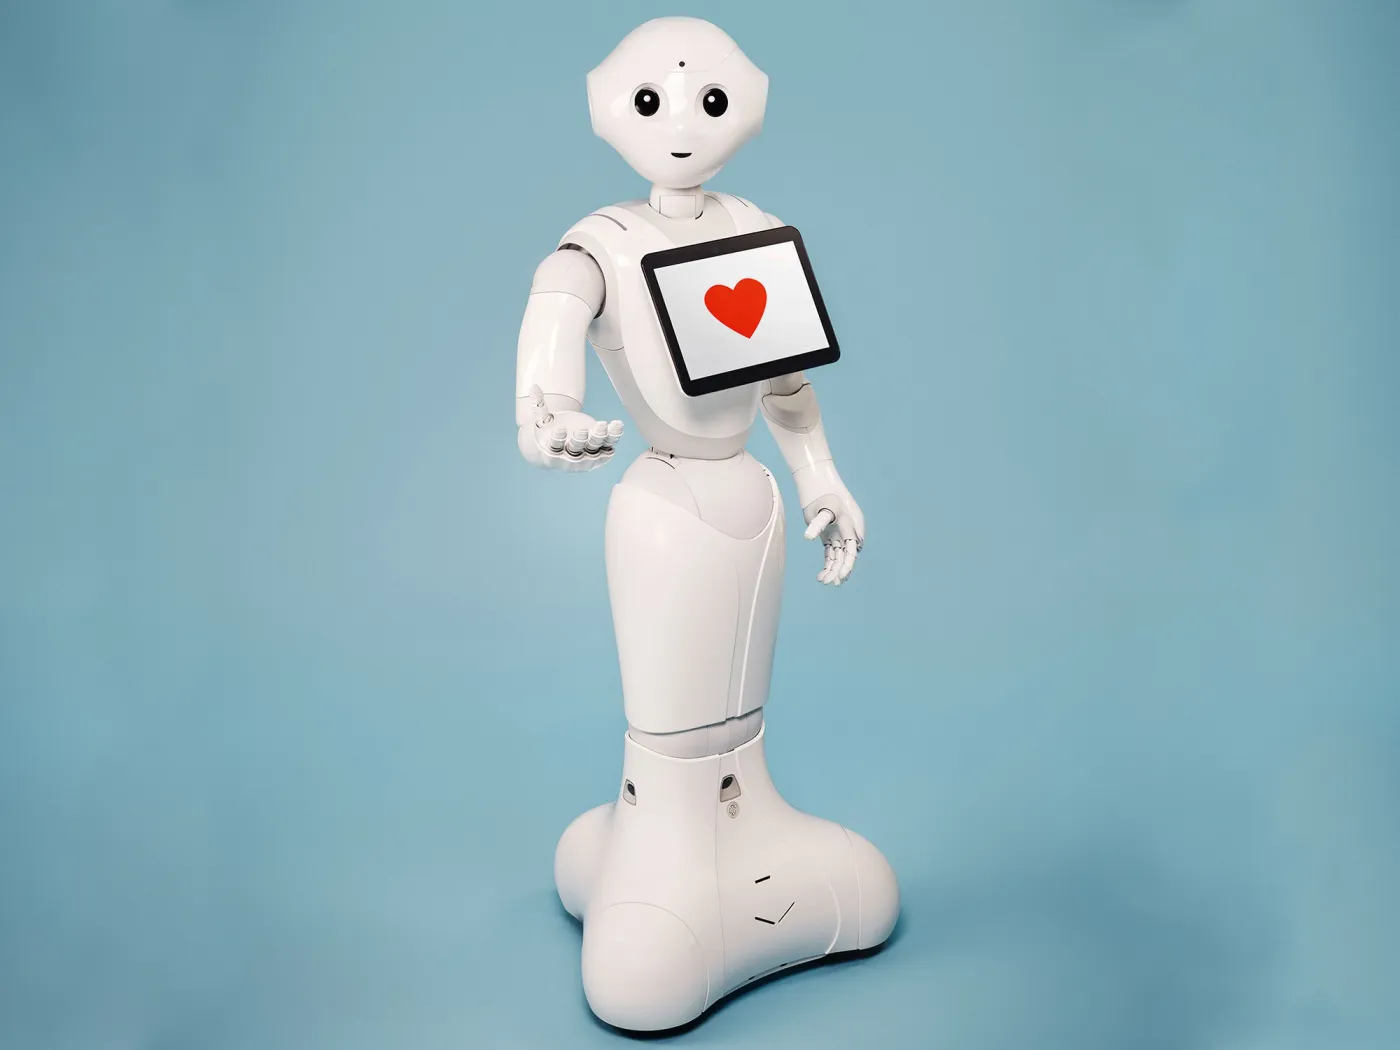
\includegraphics[width=\textwidth]{pepper.png}
    \caption{Pepper, the humanoid robot adapted from \cite{pepper2014}}
    \label{fig:pepper}
\end{figure}

\newpage
\item{\bf{Moxie}}
\vspace{0.25cm}

Moxie is an emotional support robot designed for children, especially those needing help with anxiety or emotional development. Equipped with AI and machine learning, Moxie interacts empathetically to help children build social, emotional, and cognitive skills. It engages in personalized conversations, encourages emotional expression, and uses storytelling, breathing exercises, and interactive games to foster learning. Moxie also tracks progress and adapts to each child’s needs, providing daily activities and challenges that promote emotional growth \cite{hurst2020}.

\begin{figure}[ht]
    \centering
    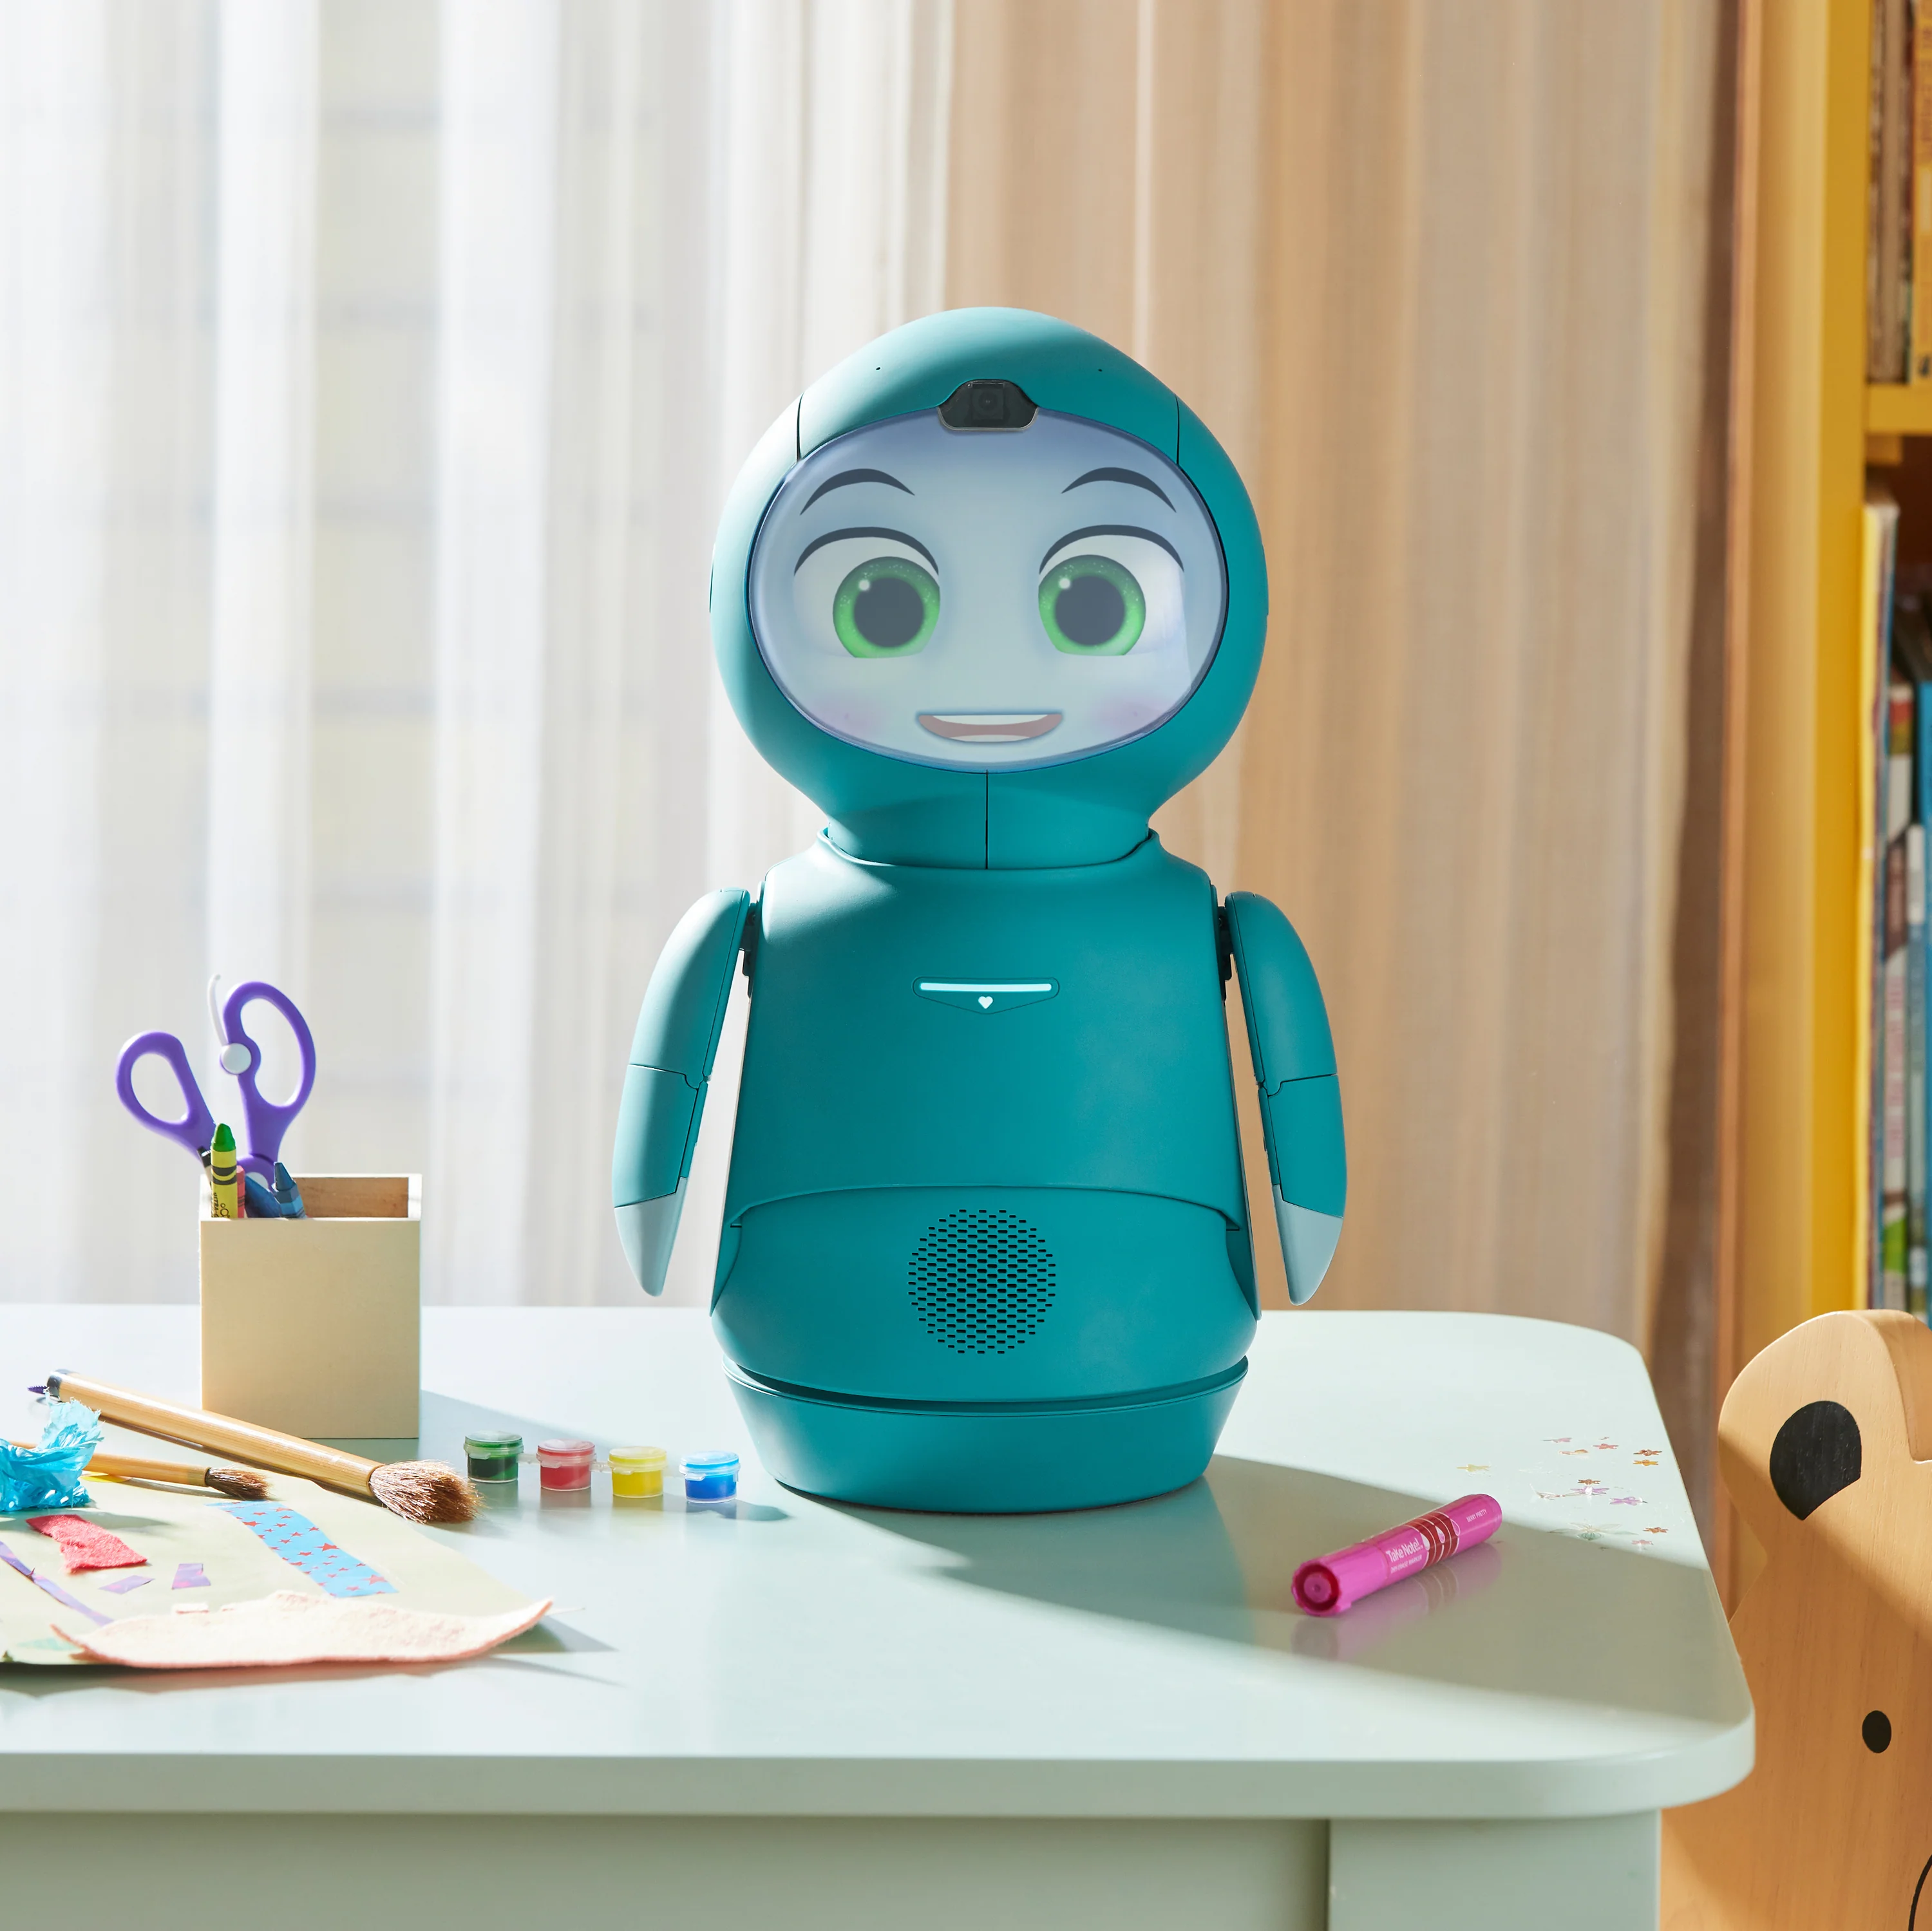
\includegraphics[width=\textwidth]{moxie.png}
    \caption{Moxie, a learning robot with heart adapted from \cite{moxie2020}}
    \label{fig:moxie}
\end{figure}

\end{enumerate}
\newpage
\subsection{State of the Art}
    
The development of mental wellbeing support robots with advanced emotional detection capabilities is an interdisciplinary endeavor that requires significant advancements in artificial intelligence (AI), robotics, and human-computer interaction (HCI). Recent research and technological progress in these areas have laid the foundation for creating robots that can not only interact with humans but also understand and respond to their emotional states. This section reviews the state of the art in emotional detection, AI-driven emotional responses, and the integration of these technologies into robotic platforms.

Emotional detection in robots is primarily driven by advancements in machine learning and deep learning techniques, particularly in the fields of computer vision, natural language processing (NLP), and speech recognition.

Facial expression recognition is a critical component, where convolutional neural networks (CNNs) are often employed to classify emotions based on facial features. Significant progress has been made in this domain with models like OpenFace \cite{baltrusaitis2018} and VGGFace \cite{zhang2023}, which offer high accuracy in identifying a wide range of emotions from facial data.

Speech-based emotion detection is another key area, where prosodic features such as tone, pitch, and rhythm are analyzed to infer emotional states \cite{swethashree2021}. Techniques like Long Short-Term Memory (LSTM) networks and more recently, transformer-based models such as BERT \cite{devlin2019}, have shown promising results in understanding the emotional content of spoken language. These models can be fine-tuned for specific languages and contexts, making them adaptable to diverse environments.

In natural language processing (NLP), sentiment analysis and emotion classification techniques are used to detect emotions from text. Advanced models like BERT \cite{wu2024} and GPT \cite{shahriar2024} have revolutionized NLP tasks, enabling the robot to understand not just the semantic content but also the emotional undertone of the conversation. This is particularly useful in chatbots and conversational agents, where understanding the user's emotions can significantly enhance the interaction quality.

Creating emotionally intelligent responses in robots involves the integration of advanced AI techniques that can interpret and respond to human emotions in a meaningful way. The development of these responses relies on recent advancements in natural language processing (NLP) and deep learning models, particularly those designed to handle the complexity of human emotions.

Transformer-based models, such as BERT and DialoGPT, have become central to generating emotionally appropriate responses. BERT, with its bidirectional encoder representations from transformers, has been extensively used in sentiment analysis tasks, enabling the model to understand and generate contextually relevant emotional responses from textual data. Research highlights the effectiveness of BERT models, especially when fine-tuned, in enhancing the accuracy and depth of emotional understanding, which is critical in generating appropriate responses \cite{wu2024}. 

DialoGPT, a model developed by Microsoft and fine-tuned on empathetic dialogue datasets, further extends these capabilities by producing responses that are not only contextually appropriate but also emotionally resonant. This model’s ability to handle nuanced emotional states and produce empathetic responses makes it particularly suited for applications in mental wellbeing support robots \cite{abuhmida2024}.

The effectiveness of these AI-driven emotional responses is often evaluated using metrics like perplexity, which measures the coherence of generated responses. Models like the transformer-based approach have demonstrated lower perplexity scores compared to others, indicating their superior ability to generate contextually and emotionally appropriate responses \cite{abuhmida2024}. Continuous optimization and fine-tuning of these models are necessary to improve their performance further, making them more reliable and effective in real-world applications.

Human-Robot Interaction (HRI) is a multidisciplinary field that encompasses various aspects of interaction between humans and robots. This field brings together knowledge from social sciences, cognitive sciences, robotics, engineering, and human-computer interaction to design, evaluate, and understand robotic systems intended for interaction with humans. The core of HRI lies in understanding how humans and robots can interact effectively, whether in a one-on-one scenario or in situations involving multiple humans and robots.

Human-robot collaboration has evolved significantly, with a focus on developing robots that can work alongside humans seamlessly. Advanced techniques such as compliance control, human performance-based approaches, model learning-based methods, and synergy models have been explored to improve collaborative interactions. These techniques allow robots to adapt to human actions, making them more responsive and effective in shared tasks \cite{safavi2024}.

Brain-Computer Interfaces (BCIs) represent a transformative approach in HRI by enabling direct communication between humans and robots through brain signals. This technology has been applied in various domains, including rehabilitation and communication, where it helps individuals with motor impairments regain control over robotic devices. The integration of BCI in HRI paves the way for more intuitive and efficient interactions, particularly in scenarios requiring real-time decision-making and adaptive responses \cite{safavi2024}.

Emotional intelligence in robotics is crucial for creating more natural and effective human-robot interactions. By recognizing and responding to human emotions through facial expressions, body gestures, and eye-tracking, robots can engage with humans on a deeper, more empathetic level. This capability is particularly important in applications such as assistive robots, where understanding and reacting to a user's emotional state can significantly enhance the interaction's quality and effectiveness \cite{safavi2024}.
